\input{einstellungen/grundeinstellungen} % Die stilistischen Parameter

\date{\today}
%---------------------------------------------------------------------------------------------------
% Anfang des Schriftstücks
%---------------------------------------------------------------------------------------------------
\begin{document}

%---------------------------------------------------------------------------------------------------
% Erstellen des Deck- und des Titelblatts
%---------------------------------------------------------------------------------------------------
\createCover{Modellierung eines Sprungs aus großer Höhe} % Art der Arbeit
{Andreas Krohn} % Author
{Hausarbeit im Rahmen der Vorlesung Modellierung technischer Systeme\\
WS2012/13 - 10.01.2012} % Title

%---------------------------------------------------------------------------------------------------
% Zusammenfassung}
%---------------------------------------------------------------------------------------------------
% \input{standard/mabstrakt.tex}

%---------------------------------------------------------------------------------------------------
% Verzeichnisse
%---------------------------------------------------------------------------------------------------
\tableofcontents % Inhaltsverzeichnis
% \listoftables % Tabellenverzeichnis
% \listoffigures % Abbildungsverzeichnis

%---------------------------------------------------------------------------------------------------
% Einführung
%---------------------------------------------------------------------------------------------------
\newpage

\section{Einführung}

Die Raumfahrt ist der Versuch der Beherrschung komplexer Technologie.
Dennoch geschehen Unfälle, die gerade in der Start- und Landephase für Gerät und Astronauten katastrophal enden.
Die letzten Unglücke mit umgekommenen Personen waren die Space Shuttles Columbia im Jahre 2003 und Challenger im Jahre 1986.
Im Falle der Challenger gibt es Stimmen, die behaupten, dass die Crew mit einem Rettungssystem hätte überleben können.
Ein Rettungszenario wäre Ausstieg, freier Fall bis in dichtere Atmosphärenschichten und Landung mittels Fallschirm.

Hierzu hat der Getränkehersteller Red Bull im Jahre 2012 medienwirksam ein Experiment finanziert.
Der Österreicher Felix Baumgartner stieg am 14.10.2012 in einer Kapsel mittels Heliumballon in eine Höhe von $39.045m$ auf (geplant waren mindestens $35.576m$) und sprang.
Neben einem großen Spektakel und neuen Rekorden wurde damit der Beweis erbracht, dass der Sprung aus derartigen Höhen möglich ist.

Im Folgenden soll das Experiment simuliert und untersucht werden, wie der Sprung aus anderen Höhen verlaufen wäre und welche Faktoren dabei eine Rolle spielen.

% Das Überschreiten vermeintlicher Grenzen gepaart mit Neugier (und die Aussicht auf Ruhm) sind ein starker Antrieb des Menschen.
% Luft- und Raumfahrt sind eine Frucht dieser Motive.
% Trotz aller Vorkehrungen werden hierbei Risiken eingegangen.
% Im Falle der Raumfahrt zwar nur von einigen wenigen Menschen, trotzdem gibt es Bestrebungen hier die Sicherheit zu erhöhen.
% Red Bull hat hierzu medienwirksam ein Experiment finanziert:
% Der Sprung des österreichischen Felix Baumgartners aus einer geplanten Höhe von 36.576m.
% Neben der Werbewirkung und dem Aufstellen neuer Rekorde sollten dabei medizinische Daten gesammelt und die Machbarkeit eines Notausstiegs von Astronauten in großer Höhe und der Rückkehr im freien Fall getestet werden.

%---------------------------------------------------------------------------------------------------
% Modellierung
%---------------------------------------------------------------------------------------------------
\section{Modellierung}\label{sec:modellierung}

Das Experiment besteht grob aus drei Phasen:
\begin{itemize}
  \item Aufstieg im Ballon
  \item Absprung und freier Fall
  \item Gebremster Fall am Fallschirm und Landung
\end{itemize}
Der Aufstieg wird im Rahmen dieser Arbeit nicht weiter betrachtet.
Interessanter ist der Fall - vor allem der ungebremste Abschnitt von Absprung bis zum Öffnen des Fallschirms.
Um dies zu simulieren, müssen relevante Kräfte und Größen berücksichtigt werden. %identifiziert und modelliert werden.

Seitenwinde und mögliche Rotation werden nicht modelliert.
Als Masse für Springer und Ausrüstung werden $140kg$ angeommen.
Auf den Springer und seine Ausrüstung wirken lediglich zwei Kräfte:
\begin{description}
  \item[$F_g$] Zur Erde hin wirkt die Gravitation.
  \item[$F_w$] Bremsend wirkt der Luftwiderstand.%, der sich bei Öffnen des Fallschirms massiv erhöht.
\end{description}

Die ausschlaggebenden Größen werden im Folgenden beschrieben.

\subsection{Gravitation}
Die Gravitation wirkt zwischen dem Springer und der Erde.
Allgemein wird hier das newtonsches Gravitationsgesetz angewendet.
\begin{equation}
F_g=G \frac{m_1 m_2}{r^2}
\end{equation}
Dabei ist $G$ die Gravitationskonstante $66.7384\times 10^{-12} \frac{m^3}{kg\ s^2}$, $m_1$ und $m_2$ die beteiligten Massen und $r$ deren Abstand.
Bis auf $r$ (der Springer bewegt sich ja auf die Erde zu) sind hier alle Größen konstant.
$r$ ist dabei gleich dem Radius der Erde $r_E$ plus der Höhe des Springers $h$ \vgl Abb.~\ref{fig:gravitation}.
\begin{figure}[h]
  \centering
  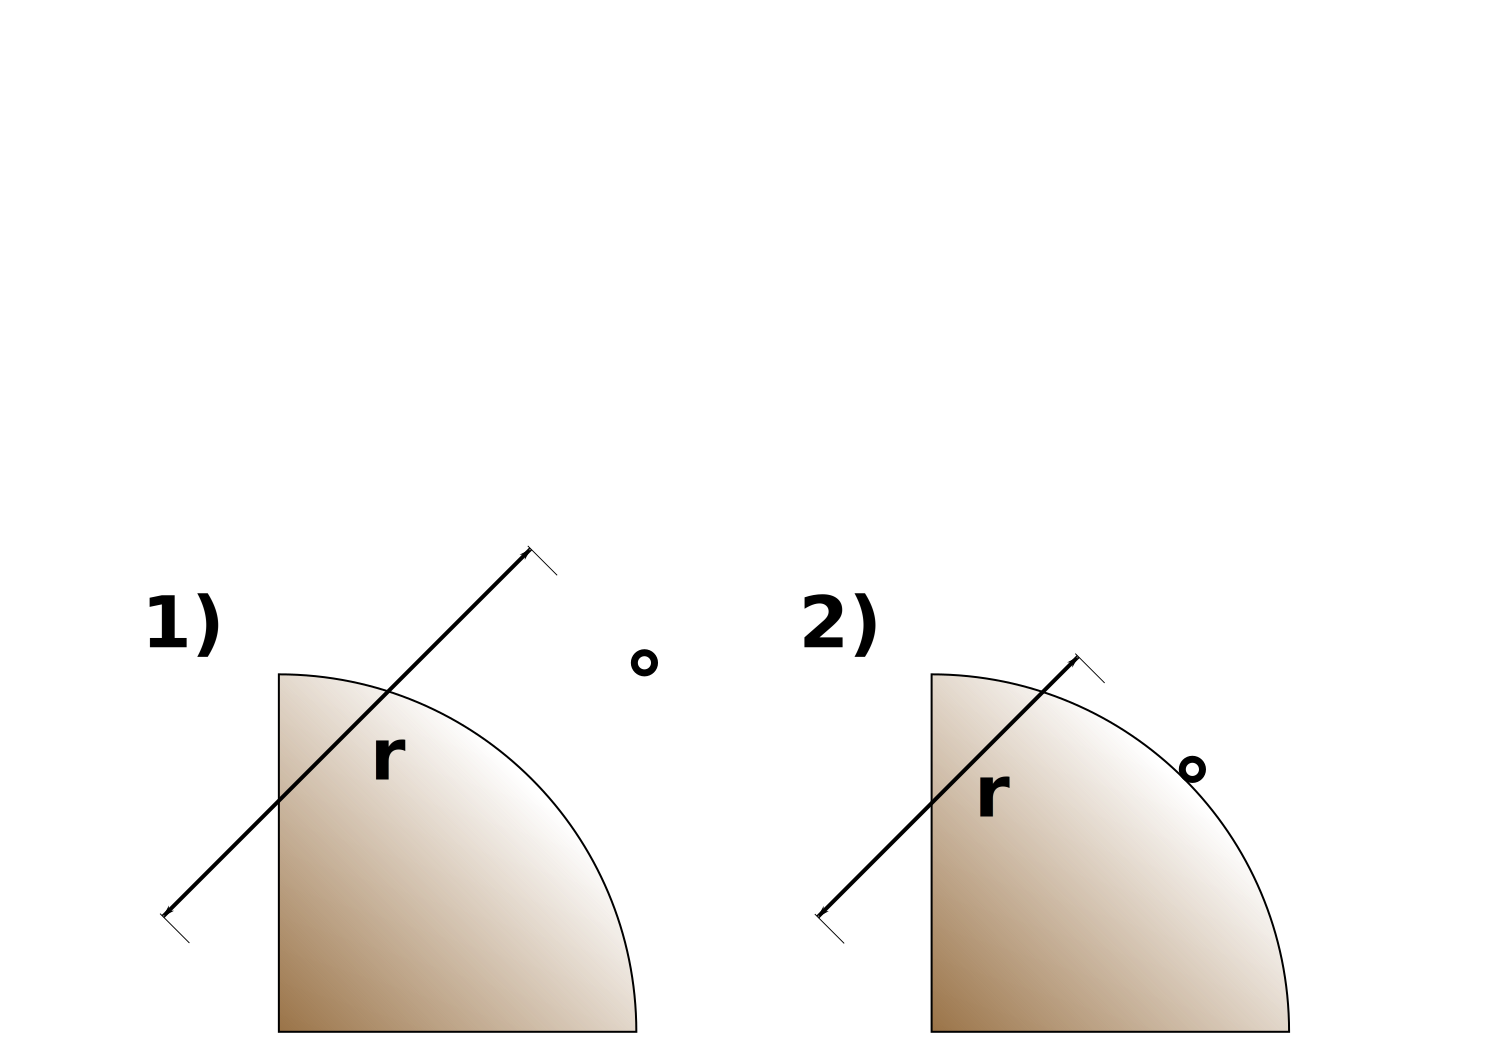
\includegraphics[width=0.5\textwidth]{gravitation}
  \caption{$r$ bei 1) Absprung und 2) Landung}
  \label{fig:gravitation}
\end{figure}

Als Erdradius wird der Äquatorradius $r_E=6 378 137m$ angenommen, als Masse des Springers $m_S=140kg$, als Masse der Erde $m_E=5.9736\times 10^{24}kg$.
Die Kraft, die auf den Springer auf Erdniveau herrscht beträgt
\begin{eqnarray}
F_{g_0} &=& 66.7384\cdot 10^{-12} \frac{140\cdot 5.9736\cdot 10^{24}}{6 378 137^2} \\
 &=& 1372 N \nonumber
\end{eqnarray}
Die Challenger zerbrach in $15km$ Höhe, der Sprung Baumgartners erfolgte aus knapp $40km$.
Um den Effekt der Höhenänderung deutlich zu zeigen wird als zweiter Wert die Gravitationskraft in $40km$ Höhe berechnet.
\begin{eqnarray}
F_{g_1} &=& 66.7384\cdot 10^{-12} \frac{140\cdot 5.9736\cdot 10^{24}}{\left(6 378 137 + 40 000\right)^2} \\
 &=& 1354.9 N \nonumber
\end{eqnarray}
Die Gravitationskraft nimmt in Absprunghöhe gegenüber der auf Erdniveau herrschenden um knapp $2\%$ ab.
Die Veränderung ist nicht groß, wird aber in der Simulation berücksichtigt.

\subsection{Luftwiderstand}
Der Fall des Springers wird durch den von der Atmosphäre verursachten Luftwiderstand gebremst.
Zur Berechnung dieser Kraft wird die Formel für den Strömungswiderstand verwendet.
\begin{equation}
F_w=\frac{1}{2}pv^2c_wA
\end{equation}
In die Berechnung der Kraft gehen die aktuelle Geschwindigkeit $v$, der Strömungswiderstandskoeffizient $c_w$, die angeströmte Fläche $A$ und die Dichte des umgebenden Mediums $p$ ein.
Die Geschwindigkeit ist das Integral der Beschleunigung, ergibt sich also zu jedem Zeitpunkt aus der Simulation.
Die Wahl von $p$, $c_w$ und $A$ werden im Folgenden beschrieben.
%Die Widerstandsfläche ändert sich bei Öffnung des Fallschirms.
%Weiterhin steigt die Widerstandsfläche in der Nähe der dichte- und temperaturabhängigen Schallgeschwindigkeit an.

\paragraph{Atmosphärenmodell}
Mit steigender Höhe nimmt der Luftdruck ab, da die darüberliegende Gassäule kürzer und somit leichter wird.
Auch die Temperatur ist höhenabhängig.
Zunächst ist die Temperatur der Erdoberfläche der ausschlaggebende Faktor.
Mit zunehmender Höhe nimmt dieser Einfluss ab und die Temperatur sinkt.
Ab einer bestimmten Höhe nimmt die Temperatur wieder zu, da ein immer geringerer Anteil der Einstrahlung von darüberliegenden Atmosphärenschichten blockiert wird.
Die Höhe, ab der die Temperatur wieder steigt ist von vielen Faktoren wie zum Beispiel der Tages- und Jahreszeit abhängig.
Nach einiger Beschäftigung mit Meteorologie, der Schichtung der Atmosphäre, Höhenformeln, virtueller Temperatur usw.~\cite{met:einfuehrung, met:umwelt}, wurde für die Simulation auf die eigene Umsetzung eines Atmosphärenmodells verzichtet.

Für die Simulation von Dichte und Temperatur wird das empirische NRLMSISE-00-Modell~\cite{nrlmsise00:goddardspaceflightcenter} verwendet, das in Matlab und Simulink als Funktion und Block zur Verfügung steht~\cite{matlab:mrlmsise-00}.
Es liefert abhängig von den Parametern Datum, Uhrzeit und geographische Position in einem Höhenbereich von $0$ bis $100km$ Werte für Dichte und Temperatur.
Für die Simulation wird lediglich die Höhe variiert und die anderen Parameter mit Ort und Zeit des Baumgartner-Experiments konstant vorbelegt.
Dichte und Temperatur stehen also jeweils als Funktion der Höhe zur Verfügung.

\paragraph{Strömungswiderstandskoeffizient und -fläche}
Der $c_w$-Wert eines Menschen liegt laut Zatsiorsky~\cite[88]{humankinetics} lageabhängig in einer Spanne von $0.35$ bis $1.36$.
Die höheren Werte gelten dabei für Lagen quer zum Luftstrom, das niedere Ende des Spektrums für Lagen längs zum Luftstrom.
Auch die angeströmte Fläche $A$ ist von der Richtung des Luftstroms abhängig.
Da Felix Baumgartner kurz nach dem Absprung in Rotation geriet und somit nicht kontinuierlich kopfüber längs zum Luftstrom fiel, werden für die Simulation die Werte $c_w=1.3$ und $A=0.8$ geschätzt, was in etwa dem in \cite{redbulletin:stratosspecialde} auf Seite 59 genannten Wert $c_w\cdot A=1.07$ entspricht.

\subsection{Gesamtmodell}

\begin{figure}[h]
  \centering
  \includegraphics[width=0.5\textwidth]{forces}
  \caption{Wirkende Kräfte}
  \label{fig:forces}
\end{figure}
Die resultierende Kraft $F_S$ (in Richtung Höhe) auf den Springer ist die Luftreibung minus der Gravitationskraft.
$F_S$ lässt sich zerlegen in das Produkt von Beschleunigung des Springers $a_S$ und Masse des Springers $m_S$.
Diese Formel nach $a_S$ umgestellt ist die für die Simulation benötigte Gesamtgleichung.
\begin{eqnarray}
  F_S &=& F_w-F_g \\
  a_Sm_S &=& F_w-F_g \nonumber \\
  a_S &=& \frac{F_w-F_g}{m_S} \label{f:a_s}\\
   &=& \frac{\frac{1}{2}pv^2c_wA-G\frac{m_Sm_E}{(r_E+h)^2}}{m_S} \nonumber
\end{eqnarray}
Nach dem Absprung erfährt der Springer also voraussichtlich zunächst eine negative Beschleunigung ($F_g\gg F_w$) bis die Geschwindigkeit weit genug gestiegen ist und er in dichtere Atmosphärenschichten gefallen ist und dort zunehmend abgebremst wird ($F_g<F_w$).



\section{Simulation}\label{sec:simulation}

Die Simulation wurde mit Hilfe von Matlab und Simulink durchgeführt.
Sie verfügt über die bereits besprochenen Attribute $c_w$-Wert, Anströmfläche $A$ und die Masse $m_S$. Weiterhin kann eine Absprunggeschwindigkeit $v_0$ und Abprunghöhe $h_0$ angegeben werden.

Die Funktion für $a_S$ (Formel~\ref{f:a_s}) wurde als Matlabfunktion (Listing~\ref{m:beschleunigung}) umgesetzt.
Eine weitere Matlabfunktion (Listing~\ref{m:c}) berechnet die Schallgeschwindigkeit in Abhängigkeit von der aktuellen Temperatur in Kelvin.

\lstinputlisting[caption={Matlabfunktion Beschleunigung},label=m:beschleunigung]{includes/beschleunigung.m}

\lstinputlisting[caption={Matlabfunktion Schallgeschwindigkeit},label=m:c]{includes/c.m}

Bei Erreichen der Höhe $0m$ wird die Simulation gestoppt.

Die Werte für Höhe, Geschwindigkeit, Beschleunigung und Schallgeschwindigkeit werden zur Analyse und Ausgabe in die aktuelle Workspace weitergegeben.

\begin{figure}[h]
  \centering
  \includegraphics[width=1\textwidth]{simulink}
  \caption{Aufbau der Simulation}
  \label{fig:simulink}
\end{figure}


%---------------------------------------------------------------------------------------------------
% Auswertung
%---------------------------------------------------------------------------------------------------
\section{Auswertung}\label{sec:auswertung}

Die Auswertung erfolgte anhand der ausgegebenen Graphen.
Wie in Abbildung~\ref{fig:speed_vs_height} zu sehen steigt die Fallgeschwindigkeit zunächst stark an.
Dabei ist das zu erreichende Maximum von der Absprunghöhe abhängig.
Liegt diese über einer Höhe von knapp $35000m$, überschreitet die Maximalgeschwindigkeit die lokale Schallgeschwindigkeit.

\begin{figure}[h]
  \centering
  \includegraphics[width=1\textwidth]{speed_vs_height}
  \caption{Geschwindigkeit und Schallgeschwindigkeit, Sprünge 24-40km Höhe}
  \label{fig:speed_vs_height}
\end{figure}

Unter der Annahme, dass für Joseph Kittinger im Jahre 1960 ähnliche Parameter galten, hat er bei seinem Sprung aus $31333m$ die Schallmauer nicht durchbrochen.
War dagegen der $c_w$-Wert günstiger, die angeströmte Fläche $A$ geringer oder die Absprungmasse $m_S$ größer könnte er es dennoch geschafft haben.

Die \textbf{nötige Absprunghöhe zum Durchbrechen der Schallmauer} liegt mit den gewählten Parametern bei $35240m$.

Weiterhin ist zu beobachten, dass sich die Geschwindigkeit unabhängig von der Absprunghöhe ab einer Höhe von ca. $15km$ bei allen Sprüngen gleich entwickelt.
Das \textbf{Auftreffen auf der Erdoberfläche} erfolgt bei allen simulierten Sprüngen mit einer Geschwindigkeit von knapp $47m/s$ oder knapp $170km/h$.

%---------------------------------------------------------------------------------------------------
% Schluss
%---------------------------------------------------------------------------------------------------
\section{Zusammenfassung}\label{sec:schluss}

......... TBD
\newpage


%---------------------------------------------------------------------------------------------------
% Literaturverzeichnis
%---------------------------------------------------------------------------------------------------
\bibliographystyle{IEEEtran} % dinat.bst fehlt, kein format für @ONLINE, gefällt mir so irgendwie besser..
\bibliography{literatur/literatur2} % Literaturverzeichnis

%---------------------------------------------------------------------------------------------------
% Ende des Schriftstücks
%---------------------------------------------------------------------------------------------------
\end{document}
